\documentclass[uplatex]{jsarticle}
\usepackage{amsmath,amssymb}
\usepackage{here}
\usepackage[dvipdfmx]{graphicx}

\title{upLatex on Docker}

\begin{document}
\maketitle

\begin{abstract}
  docker compose を使って vscodeで自動で環境生成するように変更。
\end{abstract}

\section{導入方法、起動方法}
\begin{itemize}
\item  tex(workと.devcontainerのあるディレクトリ)をVScodeで開く。  \\
(Linuxならターミナルから 「\$code .」か、 Windowsならフォルダの右クリックメニューから開く)

\item Reopen in containerを押す。(コマンドパレットから選択でも可)

\begin{figure}[H]
  \centering
  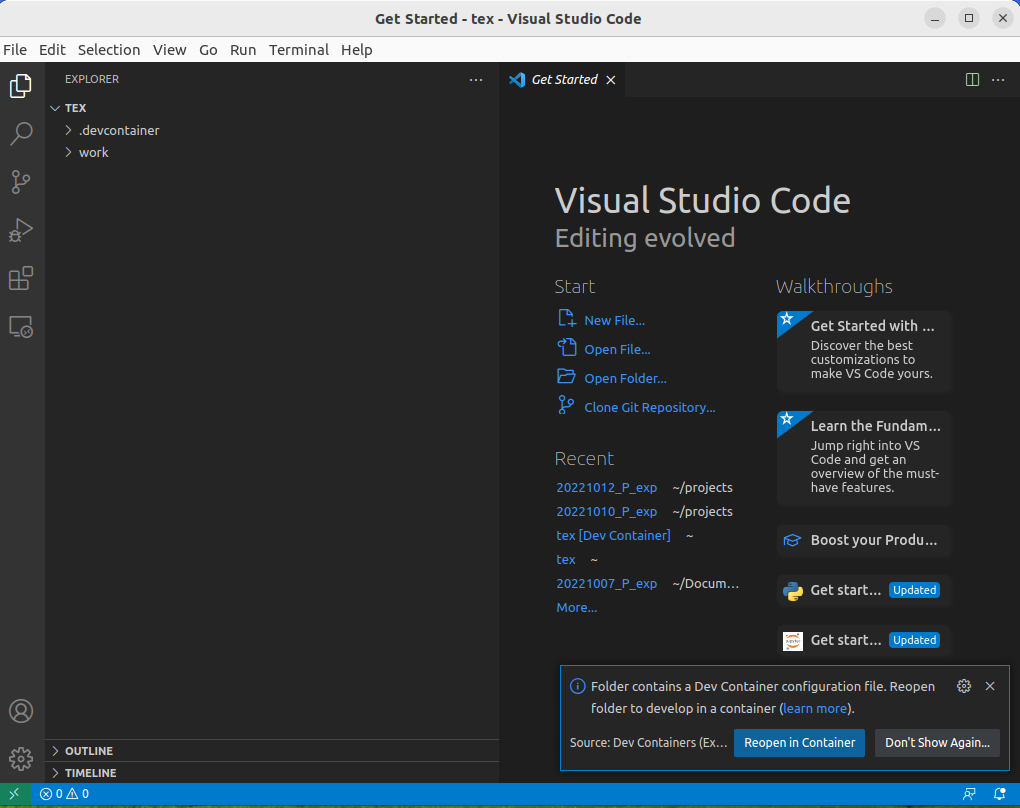
\includegraphics[width=0.7 \linewidth]{imgs/reopen_in_container.png}
  \caption{これの右下のやつ}
\end{figure}

\item 初回起動時はコンテナの生成が始まる。2回目以降はコンテナが起動する。
\end{itemize}

\section{使い方}
\begin{itemize}
\item コンテナ起動後、woekフォルダのtexファイルを選択すると、VScodeの左側に「TeX」マークでtex workshopが出てくる。
\item texファイルを保存すると、自動的にPDFが生成される。
\item texファイルを開いているときに、tex workshopのView LaTeX PDFを選ぶと右ペインにPDFファイルが表示される。
\item tex workshopの設定は、tex/work/.vscode/settings,json にあるので適宜変更する。
\end{itemize}

\begin{figure}[H]
  \centering
  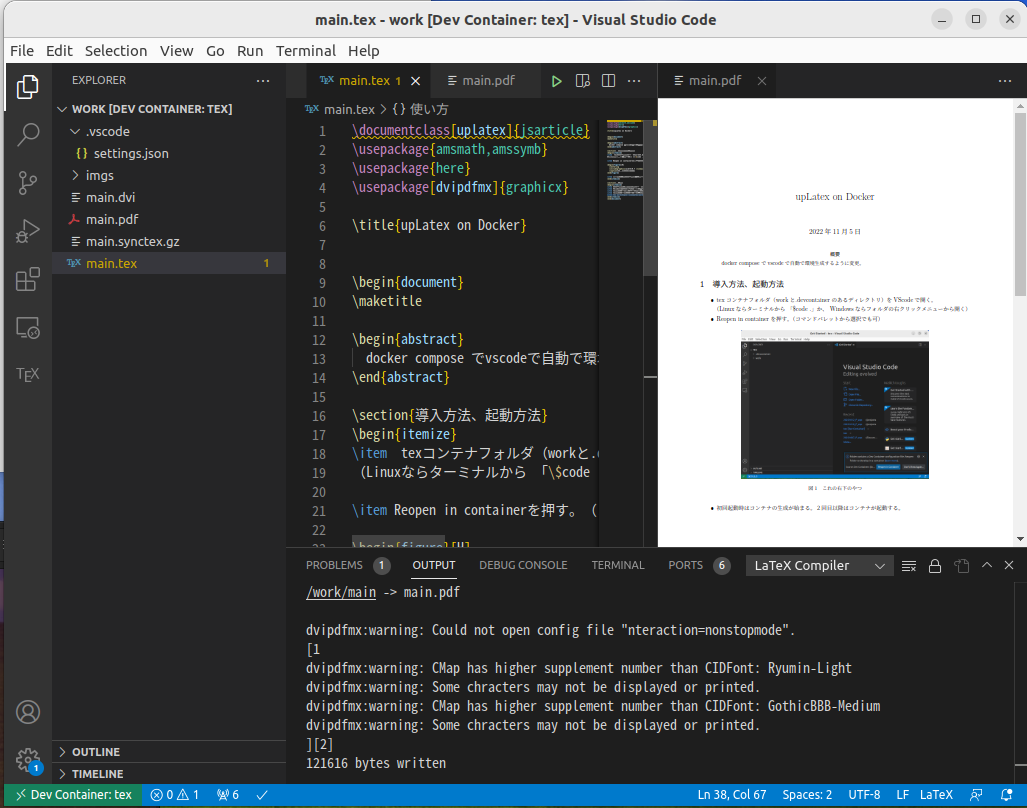
\includegraphics[width=0.7 \linewidth]{imgs/tex_workshop.png}
  \caption{tex workshopの画面}
\end{figure}

\end{document}